\documentclass[11pt, oneside]{article}
\usepackage{amsfonts}
\usepackage{amsthm}
\usepackage{amsmath}
\usepackage{setspace}
\usepackage{graphicx}
\usepackage{mathtools}
\usepackage{tikz}

\usepackage{stackengine}

\newtheorem{Question}{Question}
\newtheorem{Algorithm}{Algorithm}
\newtheorem{claim}{claim}
\graphicspath{ {images/} } %\includegraphics{name}

\usepackage{geometry}
\geometry{letterpaper, portrait, margin=1in}

\title {Design and Analysis of Algorithms Assignment 2}
\author{Harrison Lee, Alex Zhao}
\date{February 1, 2019}

\begin{document}

\maketitle

\begin{Question} (4.9)
\renewcommand{\theenumi}{\alph{enumi}}
\begin{enumerate}
\item A MBST is not always a MST\par
Given G:\par
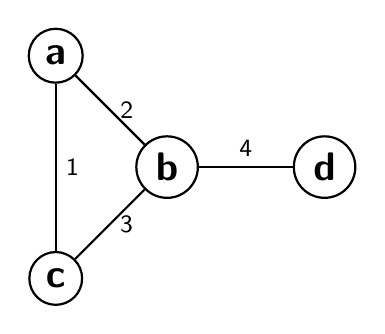
\begin{tikzpicture}[auto, node distance=2cm, every loop/.style={},
                    thick,main node/.style={circle,draw,font=\sffamily\Large\bfseries}]

  \node[main node] (1) {a};
  \node[main node] (2) [below right of=1] {b};
  \node[main node] (3) [below left of=2] {c};
  \node[main node] (4) [right of=2] {d};

  \path[every node/.style={font=\sffamily\small}]
    (1) edge node {1} (3)
    (2) edge node [right] {2} (1)
        edge node {4} (4)
    (3) edge node [right] {3} (2);
\end{tikzpicture}
\par
A MBST of G is:
\par
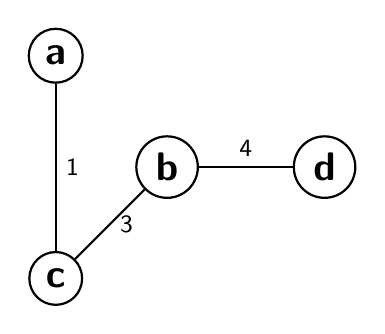
\begin{tikzpicture}[auto, node distance=2cm, every loop/.style={},
                    thick,main node/.style={circle,draw,font=\sffamily\Large\bfseries}]

  \node[main node] (1) {a};
  \node[main node] (2) [below right of=1] {b};
  \node[main node] (3) [below left of=2] {c};
  \node[main node] (4) [right of=2] {d};

  \path[every node/.style={font=\sffamily\small}]
    (1) edge node {1} (3)
    (2) edge node {4} (4)
    (3) edge node [right] {3} (2);
\end{tikzpicture}
\par
The MST of G is:
\par
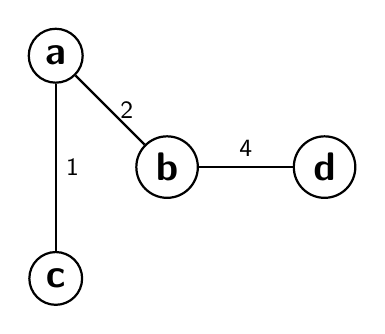
\begin{tikzpicture}[auto, node distance=2cm, every loop/.style={},
                    thick,main node/.style={circle,draw,font=\sffamily\Large\bfseries}]

  \node[main node] (1) {a};
  \node[main node] (2) [below right of=1] {b};
  \node[main node] (3) [below left of=2] {c};
  \node[main node] (4) [right of=2] {d};

  \path[every node/.style={font=\sffamily\small}]
    (1) edge node {1} (3)
    (2) edge node [right] {2} (1)
        edge node {4} (4);
\end{tikzpicture}

\item A MST is always a MBST\par
Let T be the MST of graph G. Assume that T is not the MBST $T'$ of G. That means that there is a bottleneck edge e in T not in $T'$ that is heavier than the bottleneck edge b of $T'$ (all edge weights are distinct). This means that e is heavier than every edge in $T'$. By adding e to $T'$, we create a cycle where e is the heaviest edge in this cycle. By the cycle property, this edge cannot be part of any MST. This is a contradiction. Therefore, our assumption was false and T must be a MBST. 
\end{enumerate}


\end{Question}

\newpage

\begin{Question} (6.11) Dynamic Programming
\end{Question}
\noindent Given: You have $n$ weeks and $s_i$ parts to be produced each of those weeks. You must decide between two shipping companies, Company A which charges $r * s$ to ship in a given week while Company B charges $c$ each week in blocks of four consecutive weeks.\\

\noindent Find: A schedule deciding between company A or B for each of those $n$ weeks while following company B's restrictions. Cost is the amount paid in shipping costs. \\

\noindent Give a polynomial time algorithm that takes a sequence of supply values, $s_1, s_2, \ldots , s_n$ and returns a schedule of minimum cost.

\begin{Algorithm}
Find the optimal schedule.
\end{Algorithm}

\begin{proof}
\begin{description}

Subproblems: $OPT(j)$, or the optimal schedule from week 0 to week $j$. This can be expanded from week 4 to week n.

Recurrence: $OPT(j) = min \{\stackanchor{$r * s_j + OPT(j-1)$}{$4 * c + OPT(j-4)$}$, where $OPT(j)$ represents the optimal shipping costs possible from week 0 to week $j$. $r, s,$ and $c$ are as defined in the problem, referring to company A's cost per weight unit, total weight during week $j$, and company B's cost per week respectively.

Full Algorithm: 

OPT[0, 1, 2, 3] = [0, $s_1 * r, s_1*r + s_2 * r, s_1*r + s_2*r + s_3*r$]

for j = 0, j $\leq$ n, j++

	\quad if $OPT[j - 4] + 4*c < OPT[j-1] + r*s_j$

	\quad \quad 	$OPT[j] = OPT[j-4] + 4 * c$

	\quad else:

	\quad \quad  $OPT[j] = OPT[j-1] + r*s_j$

$return OPT[n]$

Running Time: $O(n)$. Each week is traversed once, while two already calculated $OPT(j)$s are accessed, $OPT(j-1)$ and $OPT(j-4)$, each week.

\end{description}
\end{proof}


\end{document}  
